\documentclass[usenames,dvipsnames,10pt,aspectratio=169]{beamer} 

\usepackage[utf8]{inputenc}
\usepackage{verbatim}
\usepackage{minted}
\usepackage{graphicx}
\usepackage{wrapfig}
\usepackage{geometry}
\usepackage{listings}
% \usepackage{showframe}
\usepackage{enumitem}
\usepackage{color, xcolor}
\usepackage[document]{ragged2e}
\usetheme{umu}

\usemintedstyle{monokai}

\usepackage{hyperref}
\hypersetup{
    colorlinks=true,
    linkcolor=ucugreyish,
    filecolor=ucured,
    urlcolor=ucublue,
}
\urlstyle{same}

%%% Some useful commands
% pdf-friendly newline in links
\newcommand{\pdfnewline}{\texorpdfstring{\newline}{ }} 
% Fill the vertical space in a slide (to put text at the bottom)
\newcommand{\framefill}{\vskip 0pt plus 1 filll}

%%% Enter additional packages below (or above, I can't stop you)! / Jesper
\renewcommand{\proofname}{\sffamily{Proof}}

% custom fullpage image:
% { % all template changes are local to this group.
%     \setbeamertemplate{navigation symbols}{}
%     \begin{frame}<article:0>[plain]
%         \begin{tikzpicture}[remember picture,overlay]
%             \node[at=(current page.center)] {
%                 
\includegraphics[width=\paperwidth,height=\paperheight]{graphics/version-control.png}
%             };
%         \end{tikzpicture}
%      \end{frame}
% }

% custom shell example inplace
% [fragile] frame
% \begin{lstlisting}[language=Bash, style=shellstyle] 
%     username $ echo a
% \end{lstlisting}

% custom code file
% [fragile] frame
% \lstinputlisting[language=Python, style=codestyle]{code/shebang_ex.py}

% presentation template slides usage
% \framecard[color (not working)]{textbuf}
% \framesplit{Header}{picture}{textbuf}
% \framepic{image}{text}
% \lstinputlisting[language=Bash, style=codestyle]{code/namespace_ex.sh}

%%%%%%%%%%%%%%%%%%%%%%%%%%%%%%%%%%%%%%%%%%%%%%%%%%%%%%%%%%%%%%%%%%%%%%%%%%%%%%%%%%%%%
\title{Linux course}
\subtitle{Linux File systems}
\date[\today]{\small\today}
\author[Morhunenko Mykola]{Morhunenko Mykola}
\institute{APPS@UCU}

\setlist[itemize, 1]{label=$\color{ucublue} \bullet$, leftmargin=-2mm}

\begin{document}

\begin{frame}
\titlepage
\end{frame}

\begin{frame}{\contentsname}
    \setbeamercolor{background canvas}{bg=ucugrey}
    \tableofcontents
\end{frame}

\begin{frame}{Intro}
    \begin{itemize}
        \item This is not an overview of some \ex{hardware} memory staff
        \item Neither a presentation with deep File systems implementation details
        \item More about that you should learn at the \ex{Operating systems} course
        \item This is just an overview of \ex{file systems} that system administrators use in their everyday life
        \item If you think that you are not a system administrator - think one more time, because you administrate your own system every day
    \end{itemize}
\end{frame}

\section{Memory overview}
\framepic{graphics/membrain.jpg}{\hspace{-0.5cm}Memory}

\framesplit{Drives}{graphics/ssdhdd.jpeg}{
    \begin{itemize}
        \item All data stored on some physical devices
        \item It has different storage approaches on each device (HDD, SSD, CD, DVD, Flash, RAM, DDR memory modules)
        \item But now we are going to overview the memory from\ex{user point of view}
        \item How to manage files and file systems, how to choose the most suitable
    \end{itemize}
}

\framesplitc{Memory storage}{graphics/memory.png}{
    \begin{itemize}
        \item Memory as abstraction looks like an array, where bites are stored one by one in a row
        \item\ex{File system}- a method of data structure that the operating system uses to control how data is stored and retrieved
        \item A\ex{file}is an ordered collection of data blocks
        \item In Linux system, everything is a file, and if it is not a file, it is a process
        \item So File systems are very important for this OS
    \end{itemize}
}

\section{Everything is a file}
{ % all template changes are local to this group.
    \setbeamertemplate{navigation symbols}{}
    \begin{frame}<article:0>[plain]
        \begin{tikzpicture}[remember picture,overlay]
            \node[at=(current page.center)] {
                
\includegraphics[width=\paperwidth,height=\paperheight]{graphics/file.jpg}
            };
        \end{tikzpicture}
        \Huge\textbf{Everything is a file}
     \end{frame}
}

\framesplit{File types}{graphics/types.png}{
    \begin{itemize}
        \item There are a lot of file types, but the most important for us are:
        \item \ex{Regular Files} - some files with data stored inside
        \item \ex{Directories} - files, that allowed to group other files and keep tree filesystem structure
        \item \ex{Character files} - for simulating character devices as terminals, keyboard, network etc
        \item \ex{Block files} - for modelling block devices as disks, flash drives
        \item \ex{Links} - entry points to other files
        \item There are\ex{pipes}, \ex{sockets}
    \end{itemize}
}

\framesplitc{File metadata}{graphics/metha.jpg}{
    \begin{itemize}
        \item File also save a \ex{metadata} about itself, as:
        \item Protection, password
        \item Creator, owner
        \item Flags (r w x)
        \item Size 
        \item Creation time, last update time (timestamp)
    \end{itemize}
}

\begin{frame}{Inode}
    \begin{itemize}
        \item The\ex{inode}is data structure, that describes files on\ex{Unix-like OS's}
        \item Each inode stores disk block location, some atributes, file's metadata
        \item \ex{Directory}- just a file with list of inodes
        \item File's inode number can be found with\ex{ls -i}command
        \item From the inode number, the kernel's file system driver can access the inode contents, including the location of the file, thereby allowing access to the file
        \item More about\ex{inodes} in the\ex{Operating systems} course
    \end{itemize}
\end{frame}

\framesplit{Links}{graphics/symlinkvshardlink.jpeg}{
    \begin{itemize}
        \item There are two types of links:\ex{symbolic (soft)}and\ex{hard}
        \item They are totally different types of file
        \item Maybe first few years you will not use 
        \item But with experience it becomes more and more useful
        \item Here we will make only a brief overview and comparison
    \end{itemize}
}

\begin{frame}{Hard vs Soft links}
    \begin{columns}[t, totalwidth=\textwidth]
        \begin{column}{0.47\linewidth}
            {\huge Hard links}
            \begin{itemize}
                \item Exact replica of a file
                \item Share same inode with other hard links
                \item Can not be made across filesystems
                \item Changes in\ex{hl}will reflect in other files
                \item Deleting of a hardlink wil not affect other files
                \item Can links to files only
            \end{itemize}
        \end{column}

        \begin{column}{0.47\linewidth}
            {\huge Soft links}
                \begin{itemize}
                    \item Alias to a file
                    \item Has another inode 
                    \item Can be established outside filesystem
                    \item Link becomes inaccessible without original file
                    \item Can links to both files and directories
                \end{itemize}
        \end{column}
    \end{columns}
\end{frame}

\section{Fyle systems}
{ % all template changes are local to this group.
    \setbeamertemplate{navigation symbols}{}
    \begin{frame}<article:0>[plain]
        \begin{tikzpicture}[remember picture,overlay]
            \node[at=(current page.center)] {
                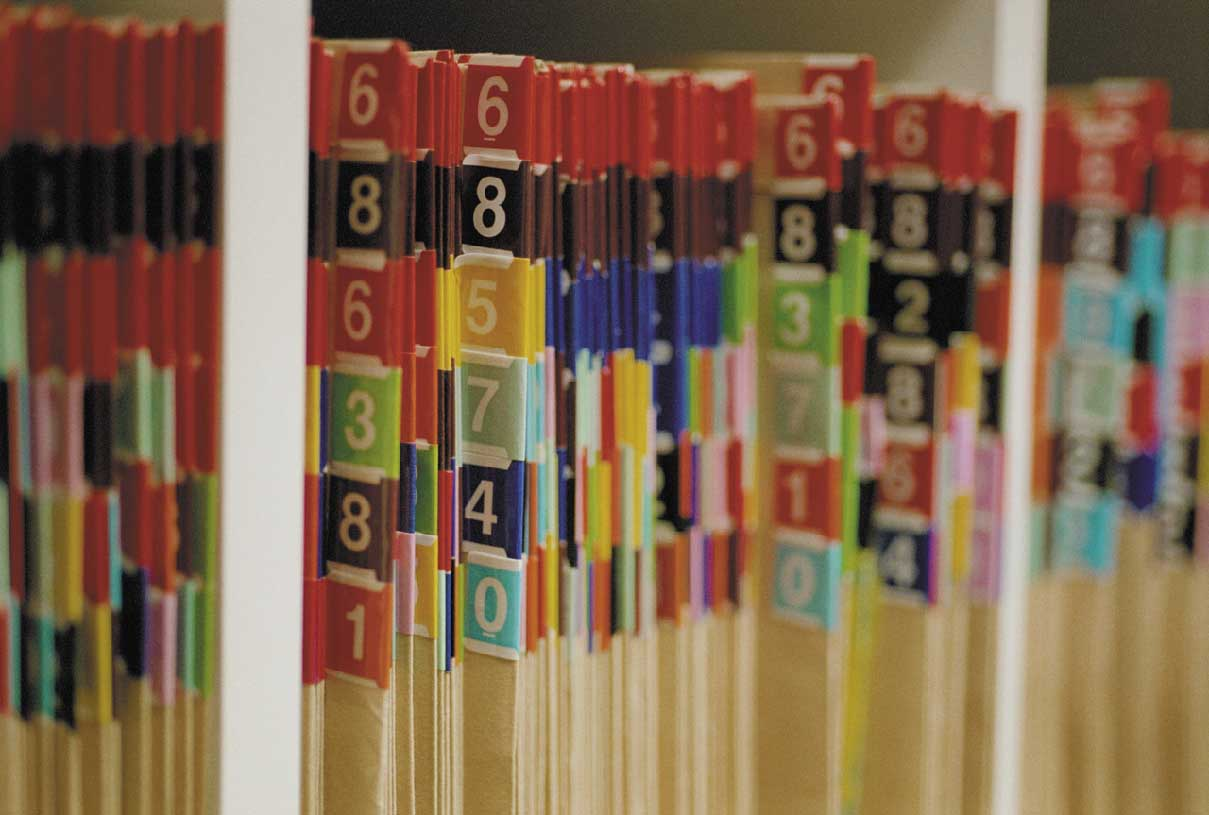
\includegraphics[width=\paperwidth,height=\paperheight]{graphics/fs.jpg}
            };
        \end{tikzpicture}
        \hspace{4cm}\Huge\textbf{File systems}
    \end{frame}
}

\begin{frame}{Fyle systems types overview}
    \begin{itemize}
        \item There are several file systems types. Just for your information. the most important will be in \ex[ucuorange]{orange} colour
        \item\ex[ucuorange]{Disk file systems} for simple disks, a.e. FAT16/32, NTFS, ext2-4, brtfs etc
        \item\ex{Flash file systems} - consider speciality of flesh memory devices
        \item\ex{Database file systems} - another concept for file management
        \item Transactional file systems
        \item\ex[ucuorange]{Network file systems} - acts as a client for a remote file access protocol, providing access to files on a server, a.e. FTP
        \item\ex{Shared disk file systems} - a number of machines (usually servers) all have access to the same external disk subsystem
        \item Flat file systems - no subdirectories, directory entries for all files are stored in a single directory
    \end{itemize}
\end{frame}

\framesplit{Fyle system abstraction}{graphics/fs_tree.png}{
    \begin{itemize}
        \item We used to see a filesystem as a tree. It is really the most comfortable structure as for now
        \item There is a CLI tool to see your filesystem structure called\ex{tree}
        \item Using such abstraction programmer works with files and directories, not with memory cells or some low level staff, but with files, directories and subdirectories
    \end{itemize}
}

\section{Working with file systems}
{ % all template changes are local to this group.
    \setbeamertemplate{navigation symbols}{}
    \begin{frame}<article:0>[plain]
        \begin{tikzpicture}[remember picture,overlay]
            \node[at=(current page.center)] {
                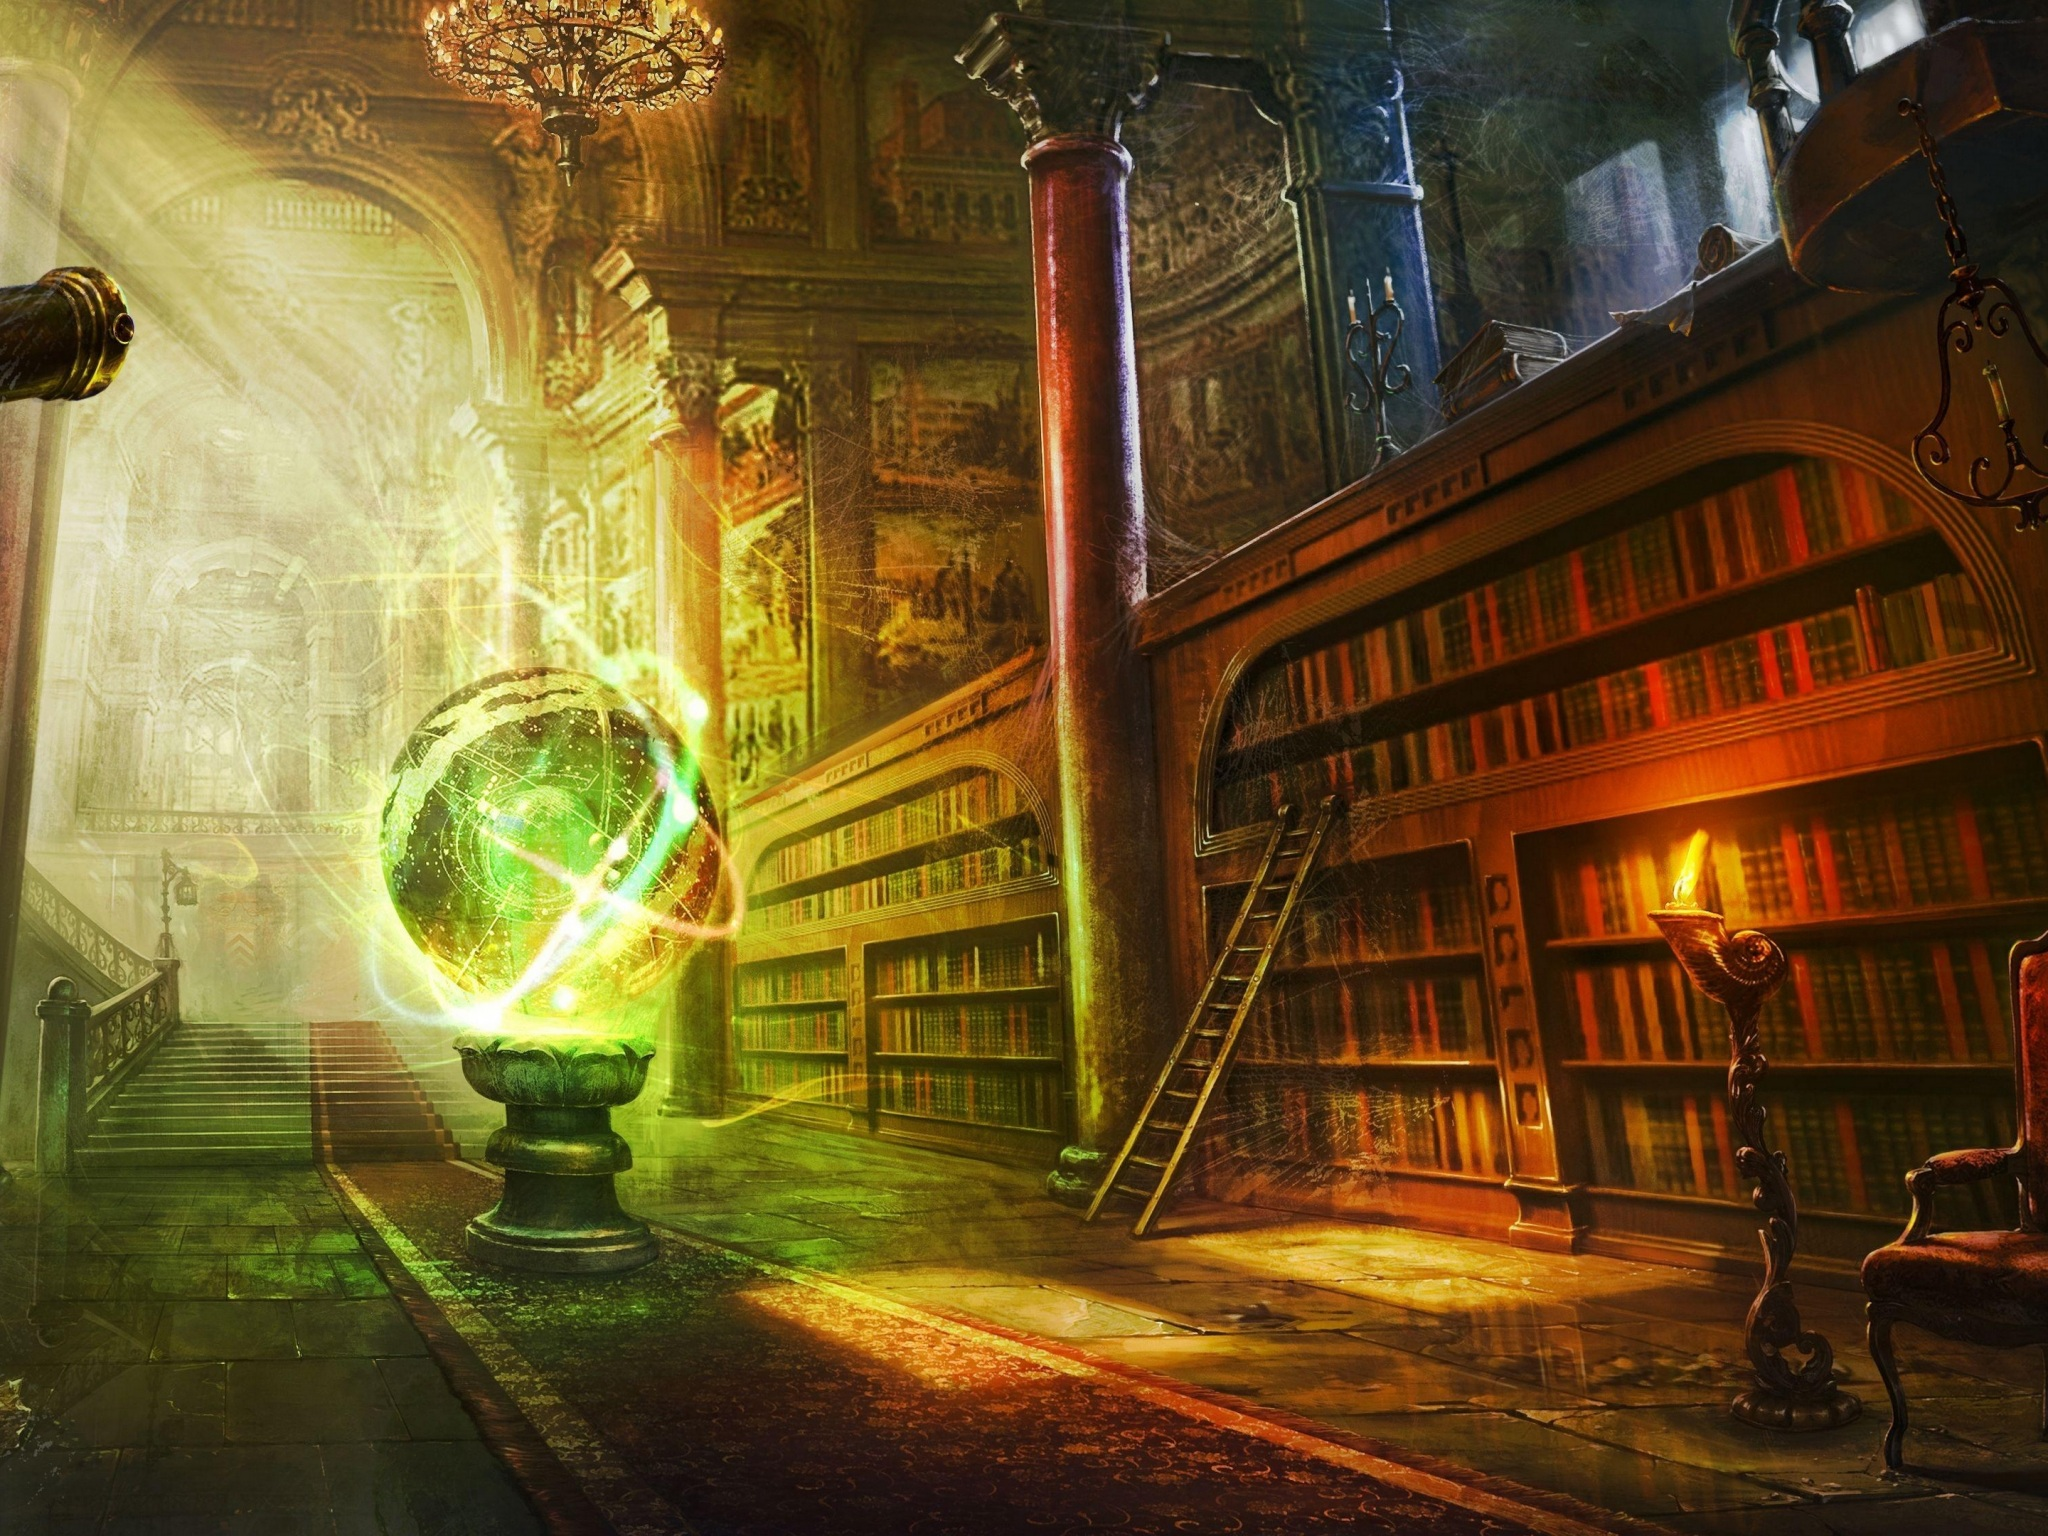
\includegraphics[width=\paperwidth]{graphics/lib.jpg}
            };
        \end{tikzpicture}
        \ex[black]{\Huge\textbf{Working with \newline\hspace{0.1em} file systems}}
     \end{frame}
}

\begin{frame}{Review of previous topics}
    \begin{itemize}
        \item It's part of presentation abot\ex{shell}, but let's make a brief overview
        \item Every proces has it's own working directory. 
        \item \ex{pwdx \$(pgrep process\_name)} - show working directories for a process\_name
        \item \ex{pwd} - print working (current) directory
        \item \ex{ls} - list what is instde the working directory
        \item \ex{cd} - change directory
        \item \ex{./} - spesial, current directory
        \item \ex{../} - spesial, parrent directory (in a tree struct)
        \item \ex{$\sim$/} - \ex{\$HOME} directory for current user
        \item \ex{cp <from....> <to>} - copy 
        \item \ex{mv <from....> <to>} - rename (inside one fs, or move - from one to another fs)
        \item \ex{mkdir} - make directory
        \item \ex{touch <filename>} - update the last acces date (if no such file - create)
        \item \ex{rm <filename>} - remove
        \item \ex{cat} - show the file content
    \end{itemize}
\end{frame}

\framesplitc{Devices}{graphics/dev.jpg}{
    \begin{itemize}
        \item \ex{Everything is a file}, devices are not an exception
        \item All devices are in\ex{/dev}folder
        \item Devices could be either\ex{secondary storages}or\ex{mous, keyboard, terminals, cpu, gpu} etc
        \item Devices can be either\ex{block}or\ex{character} devices
        \item Easy to remember:
        \item \ex{Block devices} store or hold data
        \item \ex{Character devices} - transmit or transfer data
    \end{itemize}
}

\framesplitc{Mounting}{graphics/mounts.jpeg}{
    \begin{itemize}
        \item \ex{Mounting} - attaching some additional fs to already mounted
        \item By default, user use only one filesystem, and it's mountpoint is \ex{/}
        \item Then \ex{/boot} is also another fs, that is not used by user directly (more about that\ex{bootloader} topic)
        \item On one physical device there could be few filesystems (more about that\ex{partition tables} topic)
    \end{itemize}
}

\begin{frame}{A smorgasbord of important commands and terms}
    \begin{itemize}
        \item \ex{mkfs} - make a file system on a device
        \item \ex{mkfs.filesystemtype /dev/X} - create a filesystem on existing logical device
        \item \ex{fdisk -l} - to see all devices available for mounting 
        \item \ex{mount /dev/X /mnt} - to mount device.\ex{mnt} is used as a convension, and it is important
        \item \ex{/etc/fstab}- file with all "default mountings" during startup. Usually has only \ex{/} and \ex{boot} fs's
        \item \ex{UUID} - Universally unique identifier - 128bit label. The probability that a UUID will be duplicated is close enough to zero to be negligible. HERE - unique device identifier
    \end{itemize}
\end{frame}


\section{Linux Filesystems Hierarchy (LFS)}
{ % all template changes are local to this group.
    \setbeamertemplate{navigation symbols}{}
    \begin{frame}<article:0>[plain]
        \begin{tikzpicture}[remember picture,overlay]
            \node[at=(current page.center)] {
                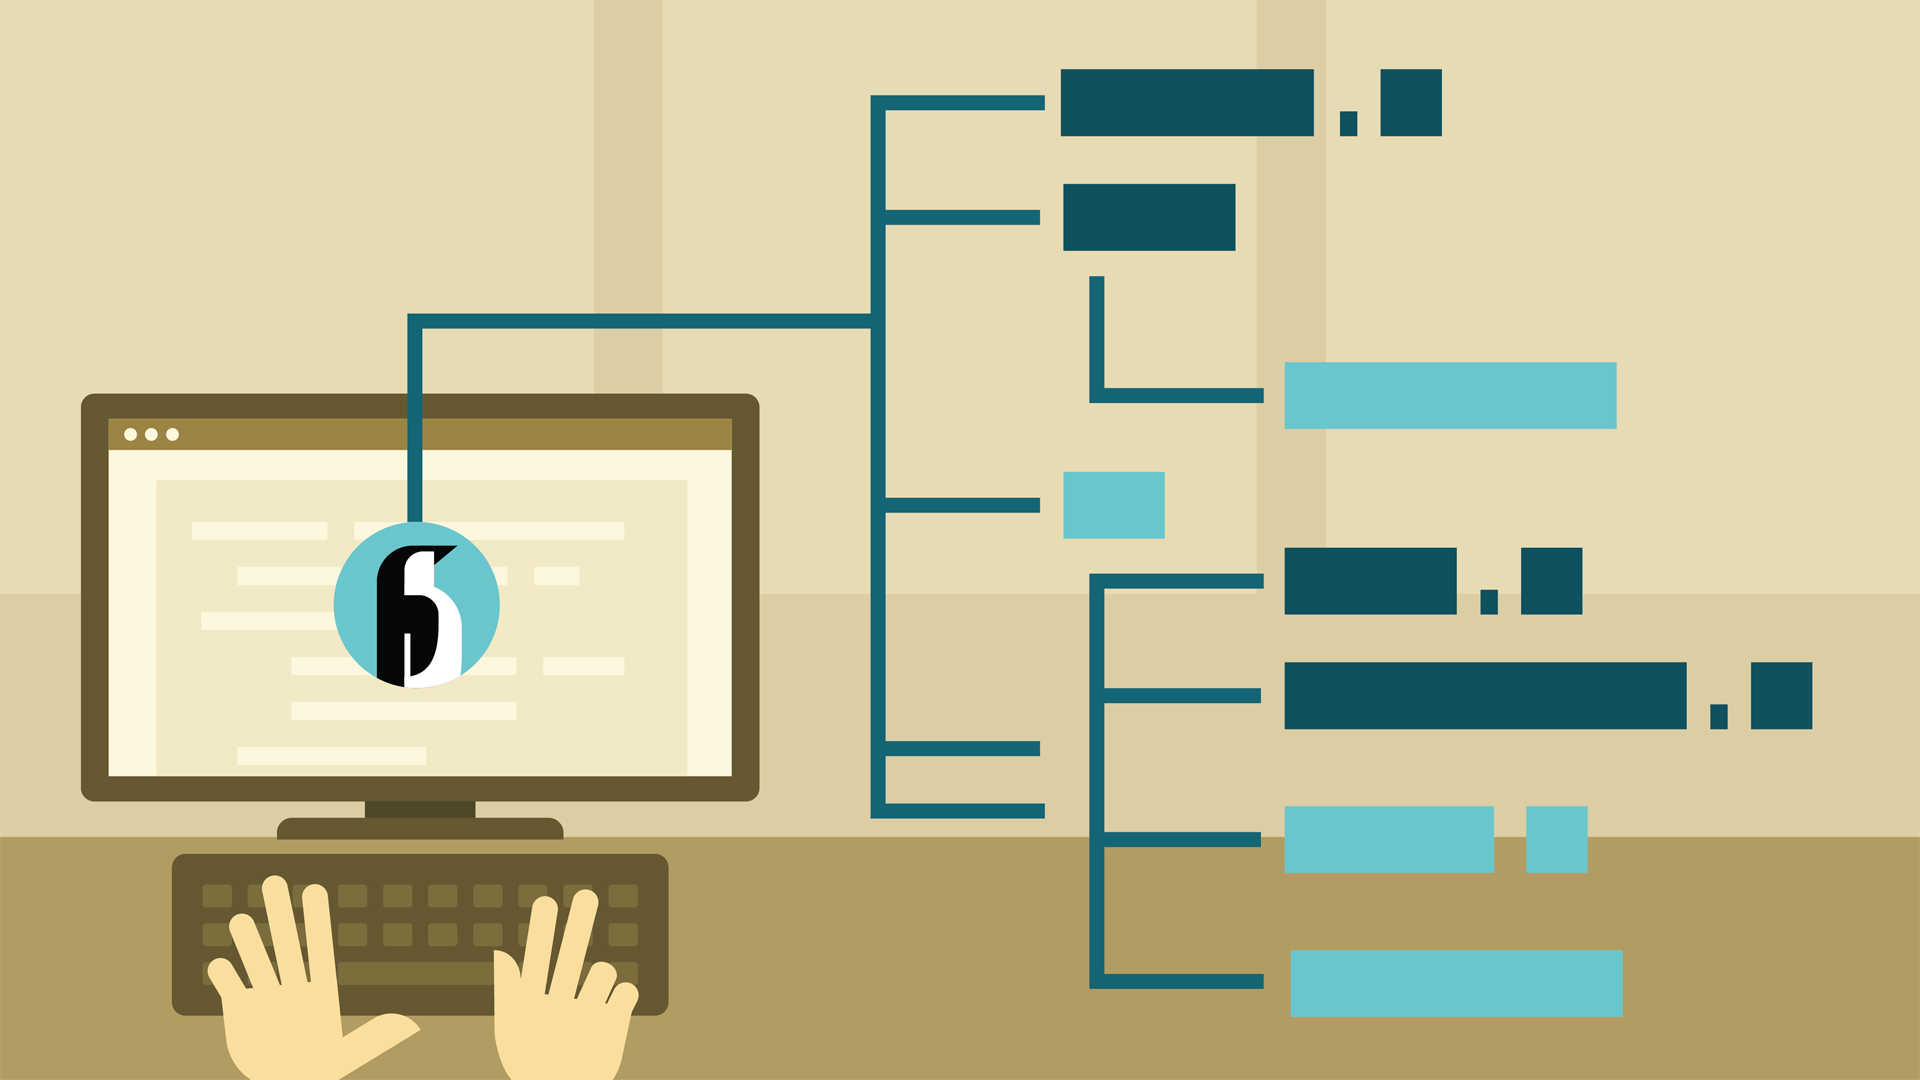
\includegraphics[width=\paperwidth,height=\paperheight]{graphics/lfs.jpg}
                % source https://www.kpl.gov/catalog/item/?i=ent://LYNDA/0/LYNDA:100016
            };
        \end{tikzpicture}
     \end{frame}
}


\begin{frame}{Linux Filesystems Hierarchy (LFS)}
    \begin{itemize}
        \item This topic worth a separate lecture, but lets make it short 
        \item 
    \end{itemize}
\end{frame}


\section{Sources}
\framecard{Sources}
\begin{frame}{Sources}
    \begin{itemize}
        \item UCU Linux Club
        \item \href{https://en.wikipedia.org/wiki/File_system}{File systems Wiki}
        \item \href{https://www.javatpoint.com/linux-files}{Linux file systems}
        \item \href{http://www.differencebetween.net/technology/difference-between-soft-link-and-hard-link-in-unix-in-os/}{Differences between hard and soft links on Unix systems}
        \item \href{https://techviewleo.com/mounting-and-unmounting-filesystems-on-linux/}{Mounting and unmounting on Linux}
        \item \href{https://en.wikipedia.org/wiki/Universally_unique_identifier}{UUID Wiki}
    \end{itemize}
\end{frame}

\end{document}